% FILE: Neuroendocrine models — HPA axis dynamics, neuroendocrine system modeling
\chapter{Neuroendocrine and Autonomic Models}
\label{ch:neuroendocrine-models}

Neuroendocrine and autonomic dysfunction contributes to many of the most debilitating symptoms of ME/CFS, including orthostatic intolerance, unrefreshing sleep, and impaired stress responses (Chapters~\ref{ch:neurological} and~\ref{ch:endocrine}). This chapter develops mathematical models of the hypothalamic--pituitary--adrenal (HPA) axis, the autonomic nervous system, and sleep--wake regulation, with emphasis on the bidirectional coupling between these systems and the immune and metabolic pathways modeled in Chapters~\ref{ch:energy-metabolism-models} and~\ref{ch:immune-system-models}.

% Figure: HPA Axis Model with ME/CFS Dysfunction
% Mathematical model diagram for Chapter 29 (Neuroendocrine Models)
% Shows cascade, feedback loops, inputs, and ME/CFS dysfunction annotations

\begin{figure}[htbp]
\centering
\resizebox{\textwidth}{!}{%
\begin{tikzpicture}[
    node distance=2.5cm and 3cm,
    >=Stealth,
    every node/.style={font=\sffamily},
    % Organ boxes
    organ/.style={
        draw=orange!70!black, fill=orange!10, very thick,
        rounded corners, text width=4.2cm, align=center,
        minimum height=1.2cm, font=\sffamily\bfseries
    },
    % Hormone labels on arrows
    hormone/.style={
        font=\sffamily\small, fill=white, inner sep=2pt
    },
    % Negative feedback arrows
    inhibit/.style={
        -Bar, thick, red!70!black, dashed
    },
    % Input arrows
    input-arrow/.style={
        -Stealth, thick, blue!70!black
    },
    % Input source box
    input-box/.style={
        draw=blue!60!black, fill=blue!5, rounded corners,
        font=\sffamily\small, text=blue!70!black,
        text width=2.8cm, align=center, minimum height=0.8cm,
        inner sep=3pt
    },
    % Input equation label
    input-eq/.style={
        font=\sffamily\scriptsize, text=blue!50!black
    },
    % ME/CFS dysfunction annotation
    mecfs/.style={
        draw=red!70!black, fill=red!8, rounded corners,
        font=\sffamily\scriptsize, text=red!70!black,
        inner sep=4pt, align=left
    },
    % Connection to immune system
    immune-box/.style={
        draw=purple!70!black, fill=purple!8, very thick,
        rounded corners, text width=3cm, align=center,
        minimum height=1cm, font=\sffamily\bfseries
    },
    % Cascade arrow
    cascade/.style={
        -Stealth, very thick, orange!70!black
    },
]

% ============================================================
% TITLE
% ============================================================
\node[font=\sffamily\large\bfseries, orange!70!black]
    (title) at (1, 1.5) {HPA Axis Model with ME/CFS Dysfunction};

% ============================================================
% MAIN CASCADE (center column)
% ============================================================

\node[organ] (hypo) at (1, 0) {Hypothalamus};
\node[organ, below=2.8cm of hypo] (pit) {Anterior Pituitary};
\node[organ, below=2.8cm of pit] (adr) {Adrenal Cortex};
\node[organ, below=2.8cm of adr, draw=orange!50!black, fill=orange!5]
    (target) {Target Tissues / Effects};

% ============================================================
% CASCADE ARROWS with hormone labels
% ============================================================

\draw[cascade] (hypo.south) -- (pit.north)
    node[hormone, midway, left=4pt] {CRH ($H$)};
\draw[cascade] (pit.south) -- (adr.north)
    node[hormone, midway, left=4pt] {ACTH ($A$)};
\draw[cascade] (adr.south) -- (target.north)
    node[hormone, midway, left=4pt] {Cortisol ($F$)};

% ============================================================
% NEGATIVE FEEDBACK LOOPS (right side)
% Feedback taps off the cortisol arrow (midway adr→target)
% Routes rightward then up, entering organ boxes from the right
% ============================================================

% Feedback tap point on cortisol arrow
\coordinate (fb-tap) at ($ (adr.south)!0.5!(target.north) $);

% --- Long loop: Cortisol → Hypothalamus ---
\draw[inhibit]
    (fb-tap) -- ++(5cm, 0) coordinate (fb-long-corner)
    |- ($ (hypo.east) + (0, 0) $);
\node[hormone, text=red!70!black, anchor=west] at (6.1, -2.5) {$K_F,\; n_F$};

% --- Short loop: Cortisol → Pituitary ---
\draw[inhibit]
    (fb-tap) -- ++(3.5cm, 0) coordinate (fb-short-corner)
    |- ($ (pit.east) + (0, 0) $);
\node[hormone, text=red!70!black, anchor=west] at (4.6, -4.5) {$K_F,\; n_{FA}$};

% Feedback annotation
\node[font=\sffamily\scriptsize, text=red!60!black, align=center]
    at (6.1, 0.8) {Negative\\feedback};

% ============================================================
% INPUTS (left side)
% ============================================================

% Circadian clock
\node[input-box] (circ) at (-3.5, 0.4)
    {Circadian clock};
\node[input-eq, below=1pt of circ]
    {$\sin(2\pi t/24 - \varphi_c)$};
\draw[input-arrow] (circ.east) -- (hypo.west |- circ.east);

% Stress
\node[input-box] (stress) at (-3.5, -0.9)
    {Stress input};
\node[input-eq, below=1pt of stress]
    {$\sigma_{\text{stress}}(t)$};
\draw[input-arrow] (stress.east) -- (hypo.west |- stress.east);

% Immune cytokines
\node[input-box] (cyto) at (-3.5, -2.2)
    {Immune cytokines};
\node[input-eq, below=1pt of cyto]
    {from immune model};
\draw[input-arrow] (cyto.east) -- ++(0.5, 0) |- ($ (hypo.south west) + (0, 0.1) $);

% ============================================================
% ME/CFS DYSFUNCTION ANNOTATIONS
% ============================================================

% At Hypothalamus: enhanced feedback sensitivity (right, near feedback)
\node[mecfs, text width=3.5cm, anchor=west] (mecfs-hypo) at (7, -1.2)
    {$\uparrow\; n_F$ enhanced\\feedback sensitivity};
\draw[red!50!black, thick, dotted, -Stealth]
    (mecfs-hypo.north) -- ++(0, 0.5) -| (fb-long-corner);

% At Circadian: blunted amplitude (left of circadian box)
\node[mecfs, text width=3cm, anchor=east] (mecfs-circ) at (-6.2, 0.4)
    {$\downarrow\; a_c$ blunted\\circadian amplitude};
\draw[red!50!black, thick, dotted, -Stealth]
    (mecfs-circ.east) -- (circ.west);

% At Stress: reduced gain (left of stress box)
\node[mecfs, text width=3cm, anchor=east] (mecfs-stress) at (-6.2, -0.9)
    {$\downarrow\; \sigma_{\text{stress}}$ gain};
\draw[red!50!black, thick, dotted, -Stealth]
    (mecfs-stress.east) -- (stress.west);

% At Cortisol output: low-normal (right, at target tissues level)
\node[mecfs, text width=3.5cm, anchor=west]
    (mecfs-cort) at (7, 0 |- target) {Low-normal cortisol\\output};
\draw[red!50!black, thick, dotted, -Stealth]
    (mecfs-cort.west) -- (target.east);

% ============================================================
% CONNECTION TO IMMUNE SYSTEM (bottom)
% ============================================================

\node[immune-box, below=2cm of target] (brake)
    {Anti-inflammatory\\Brake};
\node[immune-box, right=3cm of brake] (immune)
    {Immune System\\{\normalfont\small(Eq.~\ref{eq:cortisol-immune})}};

\draw[cascade] (target.south) -- (brake.north)
    node[hormone, midway, left=4pt] {$F$};
\draw[inhibit] (brake.east) -- (immune.west)
    node[hormone, midway, above=4pt, text=purple!70!black] {suppresses};

% ME/CFS annotation at immune connection
\node[mecfs, below=0.8cm of brake, text width=7.5cm, align=center]
    (mecfs-immune) {Weakened in ME/CFS
    $\rightarrow$ permits sustained inflammation};
\draw[red!50!black, thick, dotted]
    (mecfs-immune.north) -- (brake.south);

\end{tikzpicture}%
}% end resizebox
\caption{HPA axis feedback model (Equation~\ref{eq:hpa-axis}). The
hypothalamus--pituitary--adrenal cascade produces cortisol under circadian and
stress-driven regulation with negative feedback at hypothalamic and pituitary
levels. In ME/CFS (red annotations), enhanced feedback sensitivity, blunted
circadian amplitude, and reduced stress responsiveness produce low-normal
cortisol that inadequately restrains immune activation.}
\label{fig:hpa-axis-model}
\end{figure}


\section{HPA Axis Models}
\label{sec:hpa-axis-models}

\subsection{HPA Axis Dynamics}
\label{sec:hpa-dynamics}

The HPA axis is a neuroendocrine cascade in which the hypothalamus releases corticotropin-releasing hormone (CRH), which stimulates pituitary adrenocorticotropic hormone (ACTH) release, which in turn stimulates adrenal cortisol production. Cortisol exerts negative feedback at both the hypothalamic and pituitary levels. The model tracks three state variables---CRH ($H$), ACTH ($A$), and cortisol ($F$, from Kendall's compound~F)---with a circadian driving function:

\begin{align}
\label{eq:hpa-axis}
\frac{dH}{dt} &= \sigma_H \cdot \left(1 + a_c \sin\left(\frac{2\pi t}{24} - \phi_c\right)\right) \cdot \frac{K_F^{n_F}}{K_F^{n_F} + F^{n_F}} + \sigma_{\text{stress}}(t) - \delta_H H \\
\frac{dA}{dt} &= \sigma_A \cdot \frac{H^{n_H}}{K_H^{n_H} + H^{n_H}} \cdot \frac{K_F^{n_{FA}}}{K_F^{n_{FA}} + F^{n_{FA}}} - \delta_A A \\
\frac{dF}{dt} &= \sigma_F \cdot \frac{A}{K_A + A} - \delta_F F
\end{align}

where $\sigma_H$, $\sigma_A$, $\sigma_F$ are basal secretion rates; $a_c$ and $\phi_c$ parameterize the circadian oscillation (peak CRH release in the early morning); $K_F$ and $n_F$ control the cortisol negative feedback (Hill-type inhibition); $\sigma_{\text{stress}}(t)$ represents external stress inputs; and $\delta_H$, $\delta_A$, $\delta_F$ are degradation rates. The Hill exponents $n_F$ and $n_{FA}$ determine the sharpness of the feedback switch, with $n_F \approx 2$--$4$ producing the pulsatile cortisol release pattern observed physiologically.

\subsection{HPA Axis Dysfunction in ME/CFS}
\label{sec:hpa-dysfunction-model}

ME/CFS patients frequently exhibit subtle HPA axis abnormalities: mildly reduced basal cortisol, blunted cortisol awakening response, and attenuated cortisol response to stress~\cite{Cleare1999}. These findings are not consistent with primary adrenal insufficiency (which produces markedly low cortisol) but rather with altered central regulation. The model represents ME/CFS HPA dysfunction through three parameter modifications:

\begin{enumerate}
    \item \textbf{Enhanced negative feedback sensitivity}: increased $n_F$ (steeper Hill function), causing the system to suppress CRH output at lower cortisol concentrations. This produces the observed low-normal cortisol with preserved ACTH response.
    \item \textbf{Reduced circadian amplitude}: decreased $a_c$, flattening the diurnal cortisol rhythm. This is consistent with the blunted cortisol awakening response and may contribute to unrefreshing sleep.
    \item \textbf{Altered stress responsiveness}: reduced $\sigma_{\text{stress}}$ gain, reflecting impaired hypothalamic stress signal integration.
\end{enumerate}

The model predicts that these modifications shift the HPA axis to a low-output steady state that is stable under normal conditions but responds inadequately to metabolic or immune challenges. This has direct consequences for the immune models (Chapter~\ref{ch:immune-system-models}): cortisol is a major anti-inflammatory signal, and its deficiency permits sustained immune activation that would normally be self-limiting.

\begin{limitation}[HPA Axis Model Simplifications]
The three-variable HPA model omits several physiologically relevant features: pulsatile hormone release (ultradian rhythms with $\sim$90-minute periodicity), mineralocorticoid vs.\ glucocorticoid receptor dynamics, and cortisol-binding globulin effects on free cortisol availability. These omissions are acceptable for capturing the qualitative HPA phenotype in ME/CFS but preclude quantitative prediction of cortisol time courses at sub-hourly resolution.
\end{limitation}

% Figure: Autonomic Baroreflex and Orthostatic Intolerance Model
% Control-systems diagram for Chapter 29 (Neuroendocrine Models)

\begin{figure}[htbp]
\centering
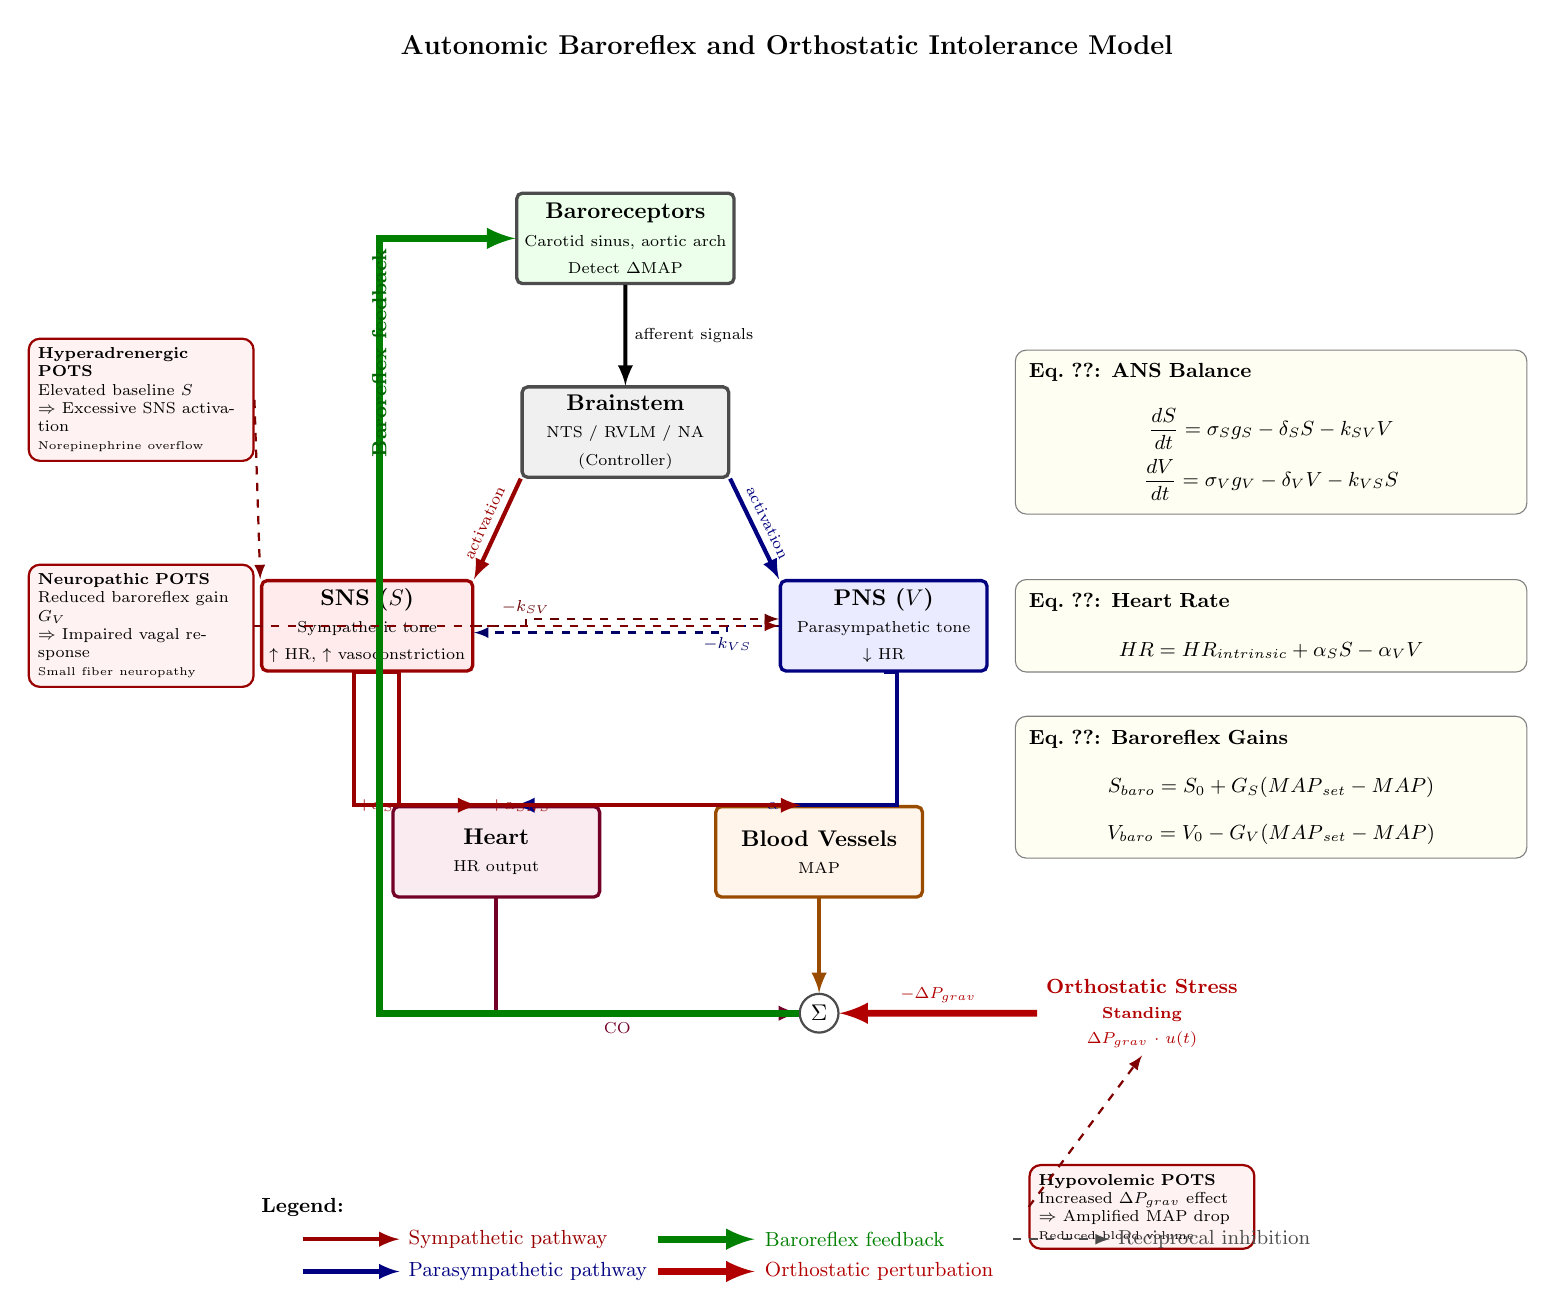
\begin{tikzpicture}[
    scale=0.82, every node/.style={scale=0.82},
    % Component styles (control-system convention)
    sensor/.style={draw=black!70, very thick, rounded corners=2pt, minimum width=3.2cm, minimum height=1.4cm, align=center, fill=green!8},
    controller/.style={draw=black!70, very thick, rounded corners=2pt, minimum width=3.2cm, minimum height=1.4cm, align=center, fill=gray!12},
    effector/.style={draw=black!70, very thick, rounded corners=2pt, minimum width=3.2cm, minimum height=1.4cm, align=center},
    sns-style/.style={effector, draw=red!60!black, fill=red!8},
    pns-style/.style={effector, draw=blue!50!black, fill=blue!8},
    heart-style/.style={effector, draw=purple!60!black, fill=purple!8},
    map-style/.style={effector, draw=orange!60!black, fill=orange!8},
    % Junction point (summing junction)
    junction/.style={circle, draw=black!70, thick, minimum size=0.6cm, inner sep=0pt, fill=white},
    % Arrow styles
    main-arrow/.style={-latex, very thick, line width=1.5pt},
    feedback-arrow/.style={-latex, ultra thick, line width=2.5pt, green!50!black},
    perturb-arrow/.style={-latex, ultra thick, line width=2.5pt, red!70!black},
    % Annotation boxes (POTS subtypes)
    pots-box/.style={draw=red!60!black, fill=red!5, rounded corners, font=\scriptsize, text width=3.2cm, align=left, inner sep=4pt, thick},
    % Equation box
    eq-box/.style={draw=black!50, fill=yellow!5, rounded corners, font=\small, inner sep=6pt, align=left},
]

% === TITLE ===
\node[font=\large\bfseries] at (2.5, 10) {Autonomic Baroreflex and Orthostatic Intolerance Model};

% === MAIN LOOP NODES ===

% Baroreceptors (top, sensor)
\node[sensor] (baro) at (0, 7) {\textbf{Baroreceptors}\\{\scriptsize Carotid sinus, aortic arch}\\{\scriptsize Detect $\Delta$MAP}};

% Brainstem (controller)
\node[controller] (brain) at (0, 4) {\textbf{Brainstem}\\{\scriptsize NTS / RVLM / NA}\\{\scriptsize (Controller)}};

% SNS (left branch)
\node[sns-style] (sns) at (-4, 1) {\textbf{SNS ($S$)}\\{\scriptsize Sympathetic tone}\\{\scriptsize $\uparrow$ HR, $\uparrow$ vasoconstriction}};

% PNS (right branch)
\node[pns-style] (pns) at (4, 1) {\textbf{PNS ($V$)}\\{\scriptsize Parasympathetic tone}\\{\scriptsize $\downarrow$ HR}};

% Heart (effector, center-left below)
\node[heart-style] (heart) at (-2, -2.5) {\textbf{Heart}\\{\scriptsize HR output}};

% MAP (effector, center-right below)
\node[map-style] (map) at (3, -2.5) {\textbf{Blood Vessels}\\{\scriptsize MAP}};

% Summing junction before MAP
\node[junction] (sum) at (3, -5) {$\Sigma$};

% === MAIN FLOW ARROWS ===

% Baro -> Brainstem
\draw[main-arrow] (baro) -- (brain) node[midway, right, font=\scriptsize] {afferent signals};

% Brainstem -> SNS (excitatory)
\draw[main-arrow, red!60!black] (brain.south west) -- (sns.north east) node[midway, above, font=\scriptsize, sloped] {activation};

% Brainstem -> PNS (excitatory)
\draw[main-arrow, blue!50!black] (brain.south east) -- (pns.north west) node[midway, above, font=\scriptsize, sloped] {activation};

% Reciprocal inhibition between SNS and PNS
\draw[-latex, thick, dashed, red!40!black] (sns.east) -- ++(0.8, 0) |- ([yshift=3pt]pns.west) node[pos=0.25, above, font=\scriptsize] {$-k_{SV}$};
\draw[-latex, thick, dashed, blue!40!black] (pns.west) -- ++(-0.8, 0) |- ([yshift=-3pt]sns.east) node[pos=0.25, below, font=\scriptsize] {$-k_{VS}$};

% SNS -> Heart
\draw[main-arrow, red!60!black] (sns.south) -- ++(-0.2,0) |- ([xshift=-8pt]heart.north) node[pos=0.7, left, font=\scriptsize] {$+\alpha_S$};

% PNS -> Heart
\draw[main-arrow, blue!50!black] (pns.south) -- ++(0.2,0) |- ([xshift=8pt]heart.north) node[pos=0.7, right, font=\scriptsize] {$-\alpha_V$};

% SNS -> Blood Vessels (vasoconstriction)
\draw[main-arrow, red!60!black] (sns.south) -- ++(0.5, 0) |- ([xshift=-8pt]map.north) node[pos=0.7, left, font=\scriptsize] {$+\alpha_{\text{SNS}}$};

% Heart -> MAP (cardiac output contributes to MAP)
\draw[main-arrow, purple!60!black] (heart.south) |- (sum.west) node[pos=0.7, below, font=\scriptsize] {CO};

% MAP output from summing junction
\draw[main-arrow, orange!60!black] (map.south) -- (sum.north);

% === FEEDBACK LOOP (Baroreflex) ===
% MAP feeds back to baroreceptors (closing the loop)
\draw[feedback-arrow] (sum.west) -- ++(-6.5, 0) |- (baro.west)
    node[pos=0.5, left, font=\small\bfseries, text=green!40!black, rotate=90] {Baroreflex feedback};

% === ORTHOSTATIC PERTURBATION ===
\node[font=\small\bfseries, red!70!black, text width=3cm, align=center] (stand) at (8, -5) {\textbf{Orthostatic Stress}\\{\scriptsize Standing}\\{\scriptsize $\Delta P_{\text{grav}} \cdot u(t)$}};
\draw[perturb-arrow] (stand) -- (sum) node[midway, above, font=\scriptsize] {$-\Delta P_{\text{grav}}$};

% === EQUATION BOXES ===

% ANS balance equation
\node[eq-box, text width=7.5cm] at (10, 4) {
    \textbf{Eq.~\ref{eq:ans-balance}: ANS Balance}
    \vspace{2pt}
    \[
    \frac{dS}{dt} = \sigma_S g_S - \delta_S S - k_{SV} V
    \]
    \vspace{-10pt}
    \[
    \frac{dV}{dt} = \sigma_V g_V - \delta_V V - k_{VS} S
    \]
};

% HR equation
\node[eq-box, text width=7.5cm] at (10, 1) {
    \textbf{Eq.~\ref{eq:heart-rate}: Heart Rate}
    \vspace{2pt}
    \[
    \text{HR} = \text{HR}_{\text{intrinsic}} + \alpha_S S - \alpha_V V
    \]
};

% Baroreflex gains
\node[eq-box, text width=7.5cm] at (10, -1.5) {
    \textbf{Eq.~\ref{eq:baroreflex}: Baroreflex Gains}
    \vspace{2pt}
    \[
    S_{\text{baro}} = S_0 + G_S(\text{MAP}_{\text{set}} - \text{MAP})
    \]
    \vspace{-10pt}
    \[
    V_{\text{baro}} = V_0 - G_V(\text{MAP}_{\text{set}} - \text{MAP})
    \]
};

% === POTS SUBTYPE ANNOTATIONS ===

% Neuropathic POTS
\node[pots-box] (pots1) at (-7.5, 1) {
    \textbf{Neuropathic POTS}\\
    Reduced baroreflex gain $G_V$\\
    $\Rightarrow$ Impaired vagal response\\
    {\tiny Small fiber neuropathy}
};
\draw[-latex, thick, red!50!black, dashed] (pots1.east) -- (pns.west);

% Hyperadrenergic POTS
\node[pots-box] (pots2) at (-7.5, 4.5) {
    \textbf{Hyperadrenergic POTS}\\
    Elevated baseline $S$\\
    $\Rightarrow$ Excessive SNS activation\\
    {\tiny Norepinephrine overflow}
};
\draw[-latex, thick, red!50!black, dashed] (pots2.east) -- (sns.north west);

% Hypovolemic POTS
\node[pots-box] (pots3) at (8, -8) {
    \textbf{Hypovolemic POTS}\\
    Increased $\Delta P_{\text{grav}}$ effect\\
    $\Rightarrow$ Amplified MAP drop\\
    {\tiny Reduced blood volume}
};
\draw[-latex, thick, red!50!black, dashed] (pots3.west) -- (stand.south);

% === LEGEND ===
\begin{scope}[yshift=-8.5cm, xshift=-5cm]
    \node[font=\small\bfseries] at (0, 0.5) {Legend:};
    \draw[main-arrow, red!60!black] (0, 0) -- (1.5, 0) node[right, font=\small] {Sympathetic pathway};
    \draw[main-arrow, blue!50!black] (0, -0.5) -- (1.5, -0.5) node[right, font=\small] {Parasympathetic pathway};
    \draw[feedback-arrow] (5.5, 0) -- (7, 0) node[right, font=\small] {Baroreflex feedback};
    \draw[perturb-arrow] (5.5, -0.5) -- (7, -0.5) node[right, font=\small] {Orthostatic perturbation};
    \draw[-latex, thick, dashed, gray!60!black] (11, 0) -- (12.5, 0) node[right, font=\small] {Reciprocal inhibition};
\end{scope}

\end{tikzpicture}
\caption{Baroreflex control loop model (Equations~\ref{eq:ans-balance}--\ref{eq:baroreflex}). Baroreceptors detect MAP changes and modulate sympathetic ($S$) and parasympathetic ($V$) tone to maintain cardiovascular homeostasis. Orthostatic stress (standing) reduces MAP, triggering compensatory responses. Three ME/CFS-associated POTS subtypes correspond to distinct parameter modifications in the model.}
\label{fig:baroreflex-model}
\end{figure}


\section{Autonomic Nervous System Models}
\label{sec:ans-models}

\subsection{Sympathetic--Parasympathetic Balance}
\label{sec:sympathetic-parasympathetic}

The autonomic nervous system (ANS) regulates cardiovascular, respiratory, and gastrointestinal function through the opposing actions of the sympathetic (SNS) and parasympathetic (PNS) branches. Heart rate variability (HRV) analysis provides a non-invasive window into ANS function and is consistently abnormal in ME/CFS~\cite{Newton2007}. The model tracks sympathetic tone ($S$) and parasympathetic (vagal) tone ($V$):

\begin{align}
\label{eq:ans-balance}
\frac{dS}{dt} &= \sigma_S \cdot g_S(\text{BP}, \text{pain}, \text{stress}) - \delta_S S - k_{SV} V \\
\frac{dV}{dt} &= \sigma_V \cdot g_V(\text{BP}, \text{respiration}) - \delta_V V - k_{VS} S
\end{align}

where $g_S$ and $g_V$ are input functions driven by baroreceptor signals (blood pressure, BP), pain, stress, and respiratory phase; $k_{SV}$ and $k_{VS}$ represent reciprocal inhibition between branches. Heart rate is determined by the balance:

\begin{equation}
\label{eq:heart-rate}
\text{HR}(t) = \text{HR}_{\text{intrinsic}} + \alpha_S \cdot S(t) - \alpha_V \cdot V(t)
\end{equation}

where $\text{HR}_{\text{intrinsic}} \approx 100$\,bpm is the intrinsic sinoatrial node rate (without autonomic input), and $\alpha_S$, $\alpha_V$ are gain coefficients. In ME/CFS, the model represents autonomic dysfunction as elevated baseline $S$ and reduced $V$---sympathetic predominance with vagal withdrawal---producing reduced HRV and elevated resting heart rate.

\subsection{Orthostatic Intolerance Model}
\label{sec:orthostatic-model}

Orthostatic intolerance (OI) affects the majority of ME/CFS patients. Upon assuming an upright posture, gravitational pooling shifts 500--700\,mL of blood to the lower extremities, requiring rapid compensatory responses. The model tracks mean arterial pressure (MAP) and heart rate during orthostatic challenge:

\begin{align}
\label{eq:orthostatic}
\frac{d\text{MAP}}{dt} &= \frac{1}{\tau_{\text{MAP}}} \left[ \text{MAP}_{\text{set}} + \alpha_{\text{SNS}} \cdot S - \text{MAP} - \Delta P_{\text{grav}} \cdot u(t) \right] \\
\frac{d\text{HR}}{dt} &= \frac{1}{\tau_{\text{HR}}} \left[ \text{HR}_{\text{intrinsic}} + \alpha_S S - \alpha_V V - \text{HR} \right]
\end{align}

where $\Delta P_{\text{grav}} \cdot u(t)$ is the gravitational pressure drop upon standing ($u(t)$ is a step function at the time of postural change), $\tau_{\text{MAP}}$ and $\tau_{\text{HR}}$ are response time constants, and $\text{MAP}_{\text{set}}$ is the baroreflex set point. The baroreflex feedback adjusts sympathetic and vagal tone in response to MAP deviations:

\begin{equation}
\label{eq:baroreflex}
S_{\text{baro}} = S_0 + G_S \cdot (\text{MAP}_{\text{set}} - \text{MAP}), \qquad V_{\text{baro}} = V_0 - G_V \cdot (\text{MAP}_{\text{set}} - \text{MAP})
\end{equation}

where $G_S$ and $G_V$ are baroreflex gains. In ME/CFS, the model represents OI through: (1)~reduced blood volume ($\Delta P_{\text{grav}}$ is amplified because the same gravitational redistribution removes a larger fraction of effective circulating volume), (2)~impaired baroreflex gain ($G_S$ and $G_V$ reduced), and (3)~excessive venous pooling (increased venous compliance in the lower extremities). The model reproduces the characteristic hemodynamic pattern of ME/CFS-associated OI: initial MAP drop, delayed or incomplete recovery, and compensatory tachycardia.

\subsection{POTS Mechanism Model}
\label{sec:pots-model}

Postural orthostatic tachycardia syndrome (POTS), defined as a sustained heart rate increase $\geq 30$\,bpm within 10 minutes of standing without orthostatic hypotension, is prevalent among ME/CFS patients. The orthostatic model (Equations~\ref{eq:orthostatic}--\ref{eq:baroreflex}) reproduces POTS when the parameter combination produces adequate MAP maintenance (through excessive sympathetic activation) at the cost of sustained tachycardia. The model identifies three parameter regimes corresponding to distinct POTS subtypes:

\begin{enumerate}
    \item \textbf{Neuropathic POTS}: reduced $G_V$ (impaired parasympathetic function) with compensatory sympathetic overdrive
    \item \textbf{Hypovolemic POTS}: reduced effective blood volume (increased $\Delta P_{\text{grav}}$ effect) requiring greater compensatory response
    \item \textbf{Hyperadrenergic POTS}: elevated baseline $S$ and increased $\alpha_S$ gain, producing excessive heart rate response to normal orthostatic stress
\end{enumerate}

This subtype classification has treatment implications: hypovolemic POTS responds to volume expansion (saline, fludrocortisone), neuropathic POTS to parasympathetic enhancement (pyridostigmine~\cite{Raj2005Pyridostigmine}), and hyperadrenergic POTS to sympatholytic agents (propranolol, clonidine).

% Figure: Tryptophan Metabolism — Serotonin vs. Kynurenine Pathway
% Branching pathway with immune modulation via IFN-gamma upregulation of IDO

\begin{figure}[htbp]
\centering
\begin{tikzpicture}[
    node distance=2.5cm and 3.5cm,
    >=latex,
    % Node styles
    input/.style={draw=green!70!black, fill=green!10, very thick, rounded corners,
        text width=4cm, align=center, minimum height=1.2cm},
    serotonin/.style={draw=blue!70!black, fill=blue!10, very thick, rounded corners,
        text width=3.8cm, align=center, minimum height=1cm},
    kynurenine/.style={draw=red!70!black, fill=red!10, very thick, rounded corners,
        text width=3.8cm, align=center, minimum height=1cm},
    enzyme/.style={draw=gray!60, fill=gray!8, rounded corners,
        text width=3.2cm, align=center, minimum height=0.9cm, font=\small},
    cofactor/.style={draw=orange!70!black, fill=orange!10, very thick, rounded corners,
        text width=3.5cm, align=center, minimum height=1cm},
    immune/.style={draw=red!80!black, fill=red!5, very thick, rounded corners,
        text width=3.5cm, align=center, minimum height=1cm},
    consequence/.style={draw=black!70, fill=yellow!8, very thick, rounded corners,
        text width=12cm, align=left, minimum height=1.5cm, font=\small},
    note/.style={font=\small\itshape, text width=3.5cm, align=center},
    arrow/.style={-latex, very thick},
    arrow-blue/.style={-latex, very thick, blue!70!black},
    arrow-red/.style={-latex, very thick, red!70!black},
    arrow-immune/.style={-latex, ultra thick, red!80!black, dashed},
]

% Title
\node[font=\large\bfseries] (title) at (0, 0)
    {Tryptophan Metabolism: Serotonin vs.\ Kynurenine Pathway};

% === Central input ===
\node[input, below=2cm of title] (trp)
    {\textbf{Tryptophan (W)}\\Essential amino acid};

% Dietary intake arrow
\node[above left=1.2cm and 2cm of trp, font=\small] (intake-label)
    {Dietary intake $I_W$};
\draw[arrow, green!70!black] (intake-label) -- (trp);

% === LEFT BRANCH: Serotonin pathway (blue) ===

% TPH enzyme
\node[enzyme, below left=2.5cm and 3cm of trp] (tph)
    {\textit{Tryptophan Hydroxylase}\\(TPH)};
\draw[arrow-blue] (trp) -- node[above left, font=\small, pos=0.4] {$v_{\mathrm{TPH}}$, $K_{\mathrm{TPH}}$} (tph);

% 5-HTP
\node[serotonin, below=2cm of tph] (htp)
    {\textbf{5-HTP}\\5-Hydroxytryptophan};
\draw[arrow-blue] (tph) -- (htp);

% Serotonin
\node[serotonin, below=2cm of htp] (serotonin)
    {\textbf{Serotonin (5-HT)}};
\draw[arrow-blue] (htp) -- (serotonin);

% Serotonin annotation
\node[note, blue!70!black, below=1.2cm of serotonin]  (sero-note)
    {Normal mood, sleep,\\pain modulation};

% === RIGHT BRANCH: Kynurenine pathway (red) ===

% IDO enzyme
\node[enzyme, below right=2.5cm and 3cm of trp] (ido)
    {\textit{Indoleamine 2,3-Dioxygenase}\\(IDO)};
\draw[arrow-red] (trp) -- node[above right, font=\small, pos=0.4] {$v_{\mathrm{IDO}}$, $K_{\mathrm{IDO}}$} (ido);

% Kynurenine
\node[kynurenine, below=2cm of ido] (kyn)
    {\textbf{Kynurenine (K)}};
\draw[arrow-red] (ido) -- (kyn);

% Quinolinic acid
\node[kynurenine, below=2cm of kyn] (quin)
    {\textbf{Quinolinic Acid}\\Neurotoxic metabolite};
\draw[arrow-red] (kyn) -- (quin);

% Kynurenine annotation
\node[note, red!70!black, below=1.2cm of quin] (kyn-note)
    {Neurotoxic metabolites\\NMDA receptor agonist};

% === IFN-gamma immune modulation ===
\node[immune, right=3cm of ido] (ifng)
    {\textbf{IFN-$\gamma$}\\Immune activation};

\draw[arrow-immune] (ifng) -- node[above, font=\small\bfseries, red!80!black] {upregulates} node[below, font=\scriptsize, red!60!black] {(Eq.~29.8)} (ido);

% Immune shift annotation
\node[note, red!80!black, text width=4cm, below=0.8cm of ifng] (shift-note)
    {\textbf{Immune activation}\\shifts balance\\W $\to$ serotonin pathway\\is suppressed};

% === BH4 cofactor ===
\node[cofactor, left=3cm of tph] (bh4)
    {\textbf{BH\textsubscript{4}}\\Tetrahydrobiopterin\\(shared cofactor)};

% BH4 to TPH
\draw[arrow, orange!70!black] (bh4) -- node[above, font=\scriptsize] {required} (tph);

% TH node for catecholamine link
\node[enzyme, below=2.5cm of bh4] (th)
    {\textit{Tyrosine Hydroxylase}\\(TH) --- catecholamines};

% BH4 to TH
\draw[arrow, orange!70!black] (bh4) -- node[left, font=\scriptsize] {required} (th);

% BH4 competition annotation
\node[note, orange!70!black, text width=3.5cm, below=1cm of th] (bh4-note)
    {Competition for BH\textsubscript{4} cofactor\\links serotonin \&\\catecholamine deficits};

% === Consequence box at bottom ===
\coordinate (bottom-mid) at ($ (sero-note.south)!0.5!(kyn-note.south) + (0, -2cm) $);
\node[consequence, anchor=north] at (bottom-mid) (consequences) {
    \textbf{ME/CFS Consequences:}\\[3pt]
    $\uparrow$ IDO activity $\;\to\;$ $\downarrow$ Serotonin + $\uparrow$ Neurotoxins
    \hfill (tryptophan steal)\\[2pt]
    Links immune activation to neuropsychiatric symptoms
    \hfill (fatigue, cognitive dysfunction, pain)
};

\end{tikzpicture}
\caption{Tryptophan metabolic branching (Equations~\ref{eq:tryptophan}--\ref{eq:ido-regulation}).
Tryptophan is metabolized through competing pathways: serotonin synthesis (left, blue) via
tryptophan hydroxylase (TPH) and kynurenine production (right, red) via indoleamine
2,3-dioxygenase (IDO). IFN-$\gamma$ from immune activation upregulates IDO, diverting
tryptophan toward neurotoxic kynurenine metabolites and depleting serotonin. BH$_4$ cofactor
competition further links this pathway to catecholamine synthesis.}
\label{fig:tryptophan-branching-model}
\end{figure}


\section{Neurotransmitter Models}
\label{sec:neurotransmitter-models}

Neurotransmitter dynamics link energy metabolism, immune function, and neurological symptoms. The tryptophan--serotonin--kynurenine axis is particularly relevant to ME/CFS because it is modulated by both immune activation and energy status.

\subsection{Tryptophan--Kynurenine Pathway}

Tryptophan is metabolized through two competing pathways: serotonin synthesis (via tryptophan hydroxylase) and kynurenine production (via indoleamine 2,3-dioxygenase, IDO). Immune activation upregulates IDO, diverting tryptophan away from serotonin toward kynurenine and its downstream neurotoxic metabolites (quinolinic acid). The model tracks tryptophan ($W$), serotonin ($5\text{HT}$), and kynurenine ($K$):

\begin{align}
\label{eq:tryptophan}
\frac{dW}{dt} &= I_W - v_{\text{TPH}} \cdot \frac{W}{K_{\text{TPH}} + W} - v_{\text{IDO}} \cdot \frac{W}{K_{\text{IDO}} + W} - \delta_W W \\
\frac{d[5\text{HT}]}{dt} &= v_{\text{TPH}} \cdot \frac{W}{K_{\text{TPH}} + W} - \delta_{5\text{HT}} [5\text{HT}] \\
\frac{dK}{dt} &= v_{\text{IDO}} \cdot \frac{W}{K_{\text{IDO}} + W} - \delta_K K
\end{align}

where $I_W$ is dietary tryptophan intake, and the IDO activity $v_{\text{IDO}}$ is upregulated by IFN-$\gamma$ from the immune model:

\begin{equation}
\label{eq:ido-regulation}
v_{\text{IDO}} = v_{\text{IDO,basal}} + v_{\text{IDO,max}} \cdot \frac{[\text{IFN-}\gamma]^2}{K_{\text{IFN}}^2 + [\text{IFN-}\gamma]^2}
\end{equation}

This coupling provides a mechanistic link between immune activation and neuropsychiatric symptoms: elevated IFN-$\gamma$ $\to$ increased IDO activity $\to$ reduced serotonin and increased neurotoxic kynurenine metabolites. The IDO metabolic trap hypothesis~\cite{phair2019ido} extends this model by proposing bistability in IDO-2 kinetics, where a high-IDO state becomes self-sustaining even after the initial immune trigger resolves. Kynurenine pathway dysregulation has been documented in ME/CFS cohorts~\cite{Kavyani2022kynurenine,Dehhaghi2022kynurenine}.

\subsection{Catecholamine Dynamics}

The NIH deep phenotyping study documented altered catecholamine metabolites in ME/CFS cerebrospinal fluid~\cite{walitt2024deep}. Catecholamines (dopamine, norepinephrine, epinephrine) are synthesized from tyrosine through a sequential enzymatic pathway. The model tracks dopamine ($\text{DA}$) and norepinephrine ($\text{NE}$) in the CNS:

\begin{align}
\label{eq:catecholamines}
\frac{d[\text{DA}]}{dt} &= v_{\text{TH}} \cdot \frac{[\text{Tyr}]}{K_{\text{TH}} + [\text{Tyr}]} \cdot \frac{[\text{BH}_4]}{K_{\text{BH}_4} + [\text{BH}_4]} - v_{\text{DBH}} \cdot \frac{[\text{DA}]}{K_{\text{DBH}} + [\text{DA}]} - \delta_{\text{DA}} [\text{DA}] \\
\frac{d[\text{NE}]}{dt} &= v_{\text{DBH}} \cdot \frac{[\text{DA}]}{K_{\text{DBH}} + [\text{DA}]} - \delta_{\text{NE}} [\text{NE}]
\end{align}

where TH is tyrosine hydroxylase (rate-limiting), DBH is dopamine $\beta$-hydroxylase, and $[\text{BH}_4]$ is tetrahydrobiopterin---a cofactor shared with tryptophan hydroxylase and nitric oxide synthase. The shared BH$_4$ dependency creates competition: increased demand for BH$_4$ by one pathway (e.g., increased NO production during inflammation) reduces availability for catecholamine and serotonin synthesis. This provides a mechanistic explanation for the concurrent monoamine deficits observed in ME/CFS.

\section{Sleep--Wake Cycle Models}
\label{sec:sleep-wake-models}

Unrefreshing sleep is a core symptom of ME/CFS. The two-process model of sleep regulation, originally developed by Borb\'{e}ly, provides a quantitative framework. Sleep propensity is determined by the interaction of a homeostatic process ($S$, sleep pressure) and a circadian process ($C$):

\begin{align}
\label{eq:sleep-wake}
\frac{dS}{dt} &= \begin{cases} r_{\text{build}} \cdot (S_{\max} - S) & \text{during waking} \\ -r_{\text{decay}} \cdot (S - S_{\min}) & \text{during sleep} \end{cases} \\
C(t) &= C_0 + C_1 \sin\left(\frac{2\pi t}{24} - \phi_s\right)
\end{align}

Sleep onset occurs when $S > C + \theta_{\text{on}}$ (sleep pressure exceeds circadian alerting plus threshold), and waking occurs when $S < C - \theta_{\text{off}}$. In ME/CFS, the model predicts unrefreshing sleep through:

\begin{enumerate}
    \item \textbf{Impaired sleep pressure dissipation}: reduced $r_{\text{decay}}$, meaning sleep pressure does not fully clear during sleep (consistent with reduced slow-wave sleep in polysomnographic studies)
    \item \textbf{Elevated waking sleep pressure build rate}: increased $r_{\text{build}}$, reflecting the higher metabolic cost of waking activities in an energy-deficient state (adenosine accumulation is linked to ATP consumption)
    \item \textbf{Blunted circadian amplitude}: reduced $C_1$, flattening the circadian alerting signal (consistent with the HPA axis circadian reduction in Section~\ref{sec:hpa-dysfunction-model} and with melatonin studies~\cite{castromarrero2021melatonin})
\end{enumerate}

The combination produces a sleep phenotype where patients fall asleep easily (elevated $S$) but wake unrefreshed (residual $S$ remains high) and experience daytime somnolence (chronically elevated $S$ during waking hours). The model further predicts that circadian disruption (irregular sleep schedules) worsens the phenotype by desynchronizing the $S$ and $C$ processes, providing formal support for sleep hygiene recommendations in ME/CFS management.

\begin{hypothesis}[Adenosine--ATP Coupling as Unrefreshing Sleep Mechanism]
The homeostatic sleep drive is mediated by extracellular adenosine, which accumulates as a byproduct of ATP hydrolysis during waking. In ME/CFS, impaired ATP production (Chapter~\ref{ch:energy-metabolism-models}) may paradoxically accelerate adenosine accumulation through increased AMP $\to$ adenosine conversion, while simultaneously impairing the glymphatic clearance of adenosine during sleep~\cite{Xie2013glymphatic,NematGorgani2025glymphatic}. This dual mechanism---accelerated build-up and impaired clearance---predicts that: (1)~sleep pressure builds faster in ME/CFS patients than in healthy controls for equivalent activity levels; (2)~improving mitochondrial function should improve sleep quality independent of sleep-targeted interventions; and (3)~glymphatic function markers should correlate with unrefreshing sleep severity.

\textbf{Certainty}: 0.35. The adenosine--ATP link is biochemically sound, but direct measurement of brain adenosine dynamics in ME/CFS patients has not been performed, and the glymphatic connection remains extrapolated from neurodegenerative disease research.
\end{hypothesis}

\section{Tetrahydrobiopterin Competition Model}
\label{sec:bh4-competition}

Tetrahydrobiopterin (BH$_4$) is an essential cofactor for three enzyme families whose products are central to ME/CFS pathophysiology: (1)~tryptophan hydroxylase (TPH, serotonin synthesis), (2)~tyrosine hydroxylase (TH, catecholamine synthesis), and (3)~all three nitric oxide synthase isoforms (eNOS, nNOS, iNOS). The shared BH$_4$ dependency was noted in the catecholamine model (Equation~\ref{eq:catecholamines}); this section formalizes the three-way competition and its consequences.

\subsection{BH$_4$ Pool Dynamics}

BH$_4$ is synthesized de novo from GTP by GTP cyclohydrolase~I (GTPCH) and regenerated from BH$_2$ by dihydrobiopterin reductase (DHFR). BH$_4$ is consumed (oxidized to BH$_2$) during each catalytic cycle of TPH, TH, and NOS:

\begin{equation}
\label{eq:bh4-dynamics}
\frac{d[\text{BH}_4]}{dt} = v_{\text{GTPCH}} + v_{\text{DHFR}} \cdot \frac{[\text{BH}_2]}{K_{\text{DHFR}} + [\text{BH}_2]} - J_{\text{TPH}} - J_{\text{TH}} - J_{\text{NOS,total}} - \delta_{\text{BH}_4} [\text{BH}_4]
\end{equation}

where $J_{\text{NOS,total}} = J_{\text{eNOS}} + J_{\text{nNOS}} + J_{\text{iNOS}}$, and iNOS activity is upregulated by pro-inflammatory cytokines (IFN-$\gamma$, TNF-$\alpha$). The conservation law $[\text{BH}_4] + [\text{BH}_2] = \text{BH}_{\text{total}}$ (neglecting de novo synthesis on fast timescales) means that increased iNOS activity during inflammation simultaneously depletes the BH$_4$ pool available to TPH and TH.

\textbf{This three-way competition produces a result that can only be derived from the mathematical model}: inflammation-driven iNOS upregulation causes coordinated deficits in serotonin (via TPH), dopamine/norepinephrine (via TH), \emph{and} endothelial NO (via eNOS uncoupling), through a single shared bottleneck. Verbal reasoning identifies each deficit independently; the model reveals that they are mechanistically linked by BH$_4$ competition and therefore cannot be corrected independently without addressing the cofactor shortage. The model predicts that:

\begin{enumerate}
    \item \textbf{BH$_4$ supplementation} (sapropterin) should simultaneously improve mood (serotonin), cognitive function (dopamine), autonomic regulation (norepinephrine), and vascular function (endothelial NO)---a prediction testable by concurrent measurement of all four downstream products
    \item \textbf{Anti-inflammatory therapy} that reduces iNOS expression should improve monoamine and NO levels even without direct neurotransmitter intervention, because it releases BH$_4$ for TPH and TH
    \item \textbf{Selective serotonin reuptake inhibitors} (SSRIs) are predicted to have reduced efficacy in ME/CFS when BH$_4$ is rate-limiting, because they increase synaptic serotonin retention but do not address the synthesis bottleneck---consistent with the generally disappointing results of antidepressants in ME/CFS
    \item The severity of concurrent serotonin, catecholamine, and NO deficits should \textbf{correlate with inflammatory burden} (IFN-$\gamma$ levels), providing a testable biomarker signature: patients with high IFN-$\gamma$ and low BH$_4$:BH$_2$ ratio should show the most severe multi-domain neurovascular dysfunction
\end{enumerate}

BH$_4$ dysregulation has been documented in ME/CFS: Gottschalk et al.\ reported elevated serum BH$_4$ levels in ME/CFS patients with orthostatic intolerance~\cite{Gottschalk2023}, which may reflect compensatory upregulation of GTPCH in response to increased NOS demand, or tissue-specific depletion masked by elevated circulating levels. The model predicts that serum BH$_4$ alone is insufficient to characterize the competition---the BH$_4$:BH$_2$ ratio and tissue-specific BH$_4$ availability are the relevant variables, and these may diverge from circulating levels when oxidative stress accelerates BH$_4$ $\to$ BH$_2$ conversion in target tissues.

\section{Cerebral Blood Flow Autoregulation}
\label{sec:cbf-autoregulation}

Reduced cerebral blood flow (CBF) is documented in ME/CFS patients, particularly during orthostatic stress~\cite{Novak2022CBFReview}. The existing cardiovascular model (Section~\ref{sec:orthostatic-model}) captures systemic hemodynamics but does not model cerebral autoregulation---the brain's ability to maintain relatively constant blood flow despite changes in systemic blood pressure. This section extends the model to capture CBF-specific dynamics.

\subsection{Cerebrovascular Autoregulation Model}

Cerebral blood flow depends on cerebral perfusion pressure (CPP) and cerebrovascular resistance (CVR):

\begin{equation}
\label{eq:cbf-model}
\text{CBF} = \frac{\text{CPP}}{\text{CVR}}, \qquad \text{CPP} = \text{MAP} - \text{ICP}
\end{equation}

where ICP is intracranial pressure ($\sim$10\,mmHg normally). Autoregulation adjusts CVR to maintain CBF constant across a MAP range of approximately 60--150\,mmHg:

\begin{equation}
\label{eq:cvr-autoregulation}
\frac{d\text{CVR}}{dt} = \frac{1}{\tau_{\text{auto}}} \left[ \text{CVR}_0 \cdot \frac{\text{MAP}}{\text{MAP}_{\text{target}}} \cdot g_{\text{CO}_2}(\text{PaCO}_2) \cdot g_{\text{NO}}([\text{NO}]) - \text{CVR} \right]
\end{equation}

where $\tau_{\text{auto}} \approx 5$--$15$\,s is the autoregulatory time constant, $\text{MAP}_{\text{target}}$ is the set point, $g_{\text{CO}_2}$ captures CO$_2$ reactivity (hypercapnia dilates cerebral vessels), and $g_{\text{NO}}$ captures NO-mediated vasodilation from the endothelial model (Equation~\ref{eq:enos-model}). In ME/CFS, the model represents impaired autoregulation through three mechanisms:

\begin{enumerate}
    \item \textbf{Delayed autoregulatory response}: increased $\tau_{\text{auto}}$, causing transient CBF undershoots during orthostatic stress before CVR adjusts
    \item \textbf{Narrowed autoregulatory range}: the MAP range over which CBF is maintained narrows, so that even moderate MAP reductions (during standing) cause CBF drops
    \item \textbf{Reduced NO-mediated vasodilation}: $g_{\text{NO}}$ is attenuated by BH$_4$ depletion (Section~\ref{sec:bh4-competition}) and endothelial dysfunction (Section~\ref{sec:coagulation-model}), impairing the vasodilatory arm of autoregulation
\end{enumerate}

\textbf{The model produces a clinically actionable prediction that requires mathematical analysis}: the CBF response to orthostatic stress depends on the product of two independent impairments (systemic MAP drop $\times$ autoregulatory delay), predicting that patients with both autonomic dysfunction (large MAP drop) and endothelial dysfunction (impaired autoregulation) will experience disproportionately severe cerebral hypoperfusion compared to patients with either alone. This multiplicative interaction explains why cognitive symptoms during orthostatic challenge are highly variable across patients with similar tilt-table hemodynamics---the cerebrovascular autoregulatory reserve differs. The model predicts that CBF ultrasound during tilt-table testing would add prognostic value beyond MAP and HR monitoring alone.

\section{Central Sensitization and Pain Amplification}
\label{sec:central-sensitization-model}

Chronic widespread pain affects the majority of ME/CFS patients and does not fully correlate with peripheral tissue damage. Central sensitization---amplification of pain signals within the spinal cord and brain---provides a mechanism for pain that persists independent of peripheral nociceptive input. This section develops a model of central sensitization that treats pain as an active feedback process rather than a passive readout.

\subsection{Spinal Cord Sensitization Dynamics}

Central sensitization is mediated by activity-dependent changes in dorsal horn neuron excitability, driven by NMDA receptor (NMDAR) activation, glial cell activation, and neuropeptide release. The model tracks the sensitization state $\mathcal{S}$ of dorsal horn circuits:

\begin{equation}
\label{eq:central-sensitization}
\frac{d\mathcal{S}}{dt} = k_{\text{wind}} \cdot P_{\text{noci}}(t) \cdot \frac{\mathcal{S}}{K_{\text{NMDA}} + \mathcal{S}} + k_{\text{glia}} \cdot \mu_{1,\text{spinal}} - k_{\text{resolve}} \cdot \mathcal{S} \cdot \frac{[\text{endorphin}]}{K_{\text{endorphin}} + [\text{endorphin}]}
\end{equation}

where $P_{\text{noci}}(t)$ is the peripheral nociceptive input (from tissue inflammation, small fiber neuropathy, or mechanical stimulation), $k_{\text{wind}}$ is the wind-up rate (NMDAR-dependent potentiation), $\mu_{1,\text{spinal}}$ is spinal glial activation (analogous to the CNS microglial model, Equation~\ref{eq:microglia}), $k_{\text{resolve}}$ is the resolution rate (modulated by endogenous opioids), and the $\mathcal{S}$-dependent term in the wind-up ensures positive feedback: existing sensitization amplifies further nociceptive input.

\subsection{Pain as a Feedback Process}

The sensitization state modifies the symptom generation function for pain (Equation~\ref{eq:symptom-mapping}):

\begin{equation}
\label{eq:pain-sensitized}
\text{Pain}(t) = (1 + \alpha_{\text{sens}} \cdot \mathcal{S}) \cdot \left[ w_4 \cdot \boldsymbol{C}_{\text{pro}}(t) + w_5 \cdot \mu_1(t) + w_6 \cdot [\text{ROS}](t) \right]
\end{equation}

where $\alpha_{\text{sens}}$ is the sensitization gain. Critically, pain itself feeds back into the system: pain increases sympathetic tone ($S$ in the ANS model, Equation~\ref{eq:ans-balance}), disrupts sleep (elevating $\theta_{\text{on}}$ in the sleep model), and consumes attentional resources (increasing effective cognitive energy demand). \textbf{This bidirectional coupling---invisible without the mathematical model---predicts that pain reduction interventions should improve not only pain but also autonomic function, sleep quality, and cognitive capacity}, because they break a feedback amplification loop. The model quantifies this: for typical ME/CFS parameters, a 50\% reduction in $\mathcal{S}$ is predicted to improve sleep efficiency by 10--15\% and reduce resting sympathetic tone by 8--12\%, mediated entirely through the pain$\to$ANS$\to$sleep pathway rather than direct effects on sleep or autonomic circuits.

Low-dose naltrexone operates in this model through two mechanisms: immune modulation (Section~\ref{sec:immune-intervention-models}) and upregulation of endogenous endorphin production (increasing $[\text{endorphin}]$ in Equation~\ref{eq:central-sensitization}), accelerating sensitization resolution. The model predicts that LDN's analgesic effect should precede its anti-inflammatory effect by the difference in timescales: endorphin upregulation (days) versus cytokine network remodeling (weeks).

\subsection{Small Fiber Neuropathy Coupling}

Small fiber neuropathy (SFN)---documented in a subset of ME/CFS patients---reduces peripheral nerve fiber density, paradoxically both reducing normal sensory input and increasing aberrant nociceptive signaling. The model represents SFN as a slow variable modifying the nociceptive input function:

\begin{equation}
\label{eq:sfn-dynamics}
\frac{d\mathcal{F}}{dt} = -k_{\text{degen}} \cdot ([\text{ROS}] + \alpha_{\text{auto}} \cdot [\text{Ab}]) + k_{\text{regen}} \cdot \frac{[\text{NGF}] \cdot [\text{ATP}]}{(K_{\text{NGF}} + [\text{NGF}])(K_{\text{ATP,regen}} + [\text{ATP}])}
\end{equation}

where $\mathcal{F}$ is small fiber density (normalizing between 0 and 1), $k_{\text{degen}}$ is the degeneration rate (driven by oxidative stress and autoantibodies), $k_{\text{regen}}$ is the regeneration rate (dependent on nerve growth factor and ATP availability), and the nociceptive input increases as fiber density decreases below a threshold: $P_{\text{noci}} = P_0 \cdot (1 + \beta_{\text{SFN}} \cdot (1 - \mathcal{F}/\mathcal{F}_0)^+)$, where $(\cdot)^+$ denotes the positive part. \textbf{The model predicts that SFN is both a consequence and an amplifier of ME/CFS}: ROS and autoantibodies (from the disease) cause fiber loss, and fiber loss increases pain signaling, which increases sympathetic tone and energy demand, worsening the underlying disease. This feedback loop explains why SFN prevalence increases with ME/CFS disease duration.

\begin{open_question}[Reversibility of Central Sensitization in ME/CFS]
Is central sensitization in ME/CFS reversible if the driving inputs (inflammation, nociception) are removed, or does prolonged sensitization produce structural changes (synaptic remodeling, glial priming) that persist independently? The model parameterizes this as the ratio $k_{\text{resolve}} / k_{\text{wind}}$: if resolution is fast relative to wind-up, sensitization reverses when inputs diminish; if resolution is slow (due to structural changes), sensitization persists as a ``pain memory.'' This distinction has direct treatment implications: reversible sensitization responds to anti-inflammatory and analgesic therapy, while structurally maintained sensitization may require neuromodulatory interventions (NMDAR antagonists, transcranial stimulation) targeting the dorsal horn directly.
\end{open_question}
